\documentclass[a0,sans]{esatposter}
\usepackage{lmodern}
\usepackage{latexsym}           %LateX Symbol Fonts
\usepackage{graphicx}
\usepackage[dvips]{epsfig}      %Encapsulated PostScript
\usepackage{amsmath,amsfonts}
\usepackage{amssymb,wasysym,pifont}
\usepackage{multirow}
\usepackage{multicol}
\usepackage{wrapfig}
\usepackage{fixltx2e}
\usepackage{varwidth}
\usepackage{lipsum}
\usepackage{algorithm}
\usepackage[noend]{algpseudocode}
\usepackage{tikz}
\usetikzlibrary{arrows}

\graphicspath{{figures/}}


\newcommand{\bs}[1]{\boldsymbol{#1}}

\title{ \Huge Incrementally Learn the Relevance of Words in a Dictionary for Spoken Language Acquisition}
\author{ \LARGE Vincent Renkens$^1$, Vikrant Tomar$^2$, Hugo Van hamme$^1$}  \affiliation{\LARGE $^1$Department ESAT, KULeuven Belgium\\
$^2$Fluent.ai Canada}
\contact{\Large \tt vincent.renkens@esat.kuleuven.be}
\definecolor{textback}{rgb}{0.88,0.94,1}
\definecolor{BrickRed}{RGB}{128,0,0}
\definecolor{Green}{RGB}{0,128,0}
\definecolor{DarkBlue}{RGB}{0,0,128}
\newcommand{\comm}[1]{\texttt{\textbackslash #1}}
\renewcommand{\textboxbodyfont}{\large}
\renewcommand{\textboxtitlefont}{\LARGE}
\renewcommand{\section}[1]{\vspace{\stretch{2}}\par \LARGE \begin{center} \textcolor{kulblue}{\underline{\textbf{#1}}} \end{center}\large \vspace{\stretch{2}}\par}

\begin{document}

\tikzstyle{element}=[shape=rectangle,draw,align=center, minimum width = 1cm, minimum height = 2cm, fill=kulblue!80, text=white]

\maketitle

\rframe{.3}{1}
{%
	\rtextbox{.3}{.1}{1. Features}
	{%
		\vspace{-1cm}
		\large{
		\begin{itemize}
			\item Adaptively learn a set of words from a user
			\item Adapt the size of the learned set as new data is presented
		\end{itemize}}
	}\vbs
	\rtextbox{.3}{.2}{2. Application}
	{%
		\center{\textbf{A command-and-control interface that learns through interaction with the user}}
		
		\vspace{1cm}
		
		\begin{tikzpicture}
			\node[element] (command) at (0,0) {\textbf{Command}};
			\node[element] (recognition) at (8,0) {\textbf{Recognition}};
			\node[element] (demonstrate) at (16,0) {\textbf{Demonstrate}};
			\node[element] (update) at (8,-4) {\textbf{Update model}};
			\draw[->, line width=3pt] (command) -- (recognition);
			\draw[->, red, line width=3pt] (recognition) -- (demonstrate);
			\draw[->, green, line width=3pt] (recognition) -- (update);
			\draw[->, line width=3pt] (demonstrate) -- (16,-4) -- (update);
			\draw[->, line width=3pt] (update) -- (0,-4) -- (command);
		\end{tikzpicture}
		
	}\vbs
	\rtextbox{.3}{.7}{2. Weakly supervised NMF}
	{%
		\large{
			NMF: Nonnegative Matrix Factorisation
			\vspace{1cm}
			\begin{align}
				\begin{bmatrix}
					\bs{V}^\text{s}\\
					\bs{V}^\text{a}
				\end{bmatrix}
				\approx
				\begin{bmatrix}
					\bs{W}^\text{s}\\
					\bs{W}^\text{a}
				\end{bmatrix}
				\bs{H}
				\nonumber
			\end{align}
		}
		
		\large{
		\begin{itemize}
			\item $\bs{V}^\text{a}$: Acoustic data: phone bigram counts (DNN phone recognizer)
			\item $\bs{V}^\text{s}$: Semantic data: semantic representation of demonstration
			\item $\bs{W}^\text{a}$: Acoustic dictionary: recurring acoustic patterns (words)
			\item $\bs{W}^\text{s}$: Semantic dictionary: semantic representation of words
			\item $\bs{H}$: Word activations in each utterance
		\end{itemize}}
			
		\vspace{2cm}
		\hspace{-5cm}
		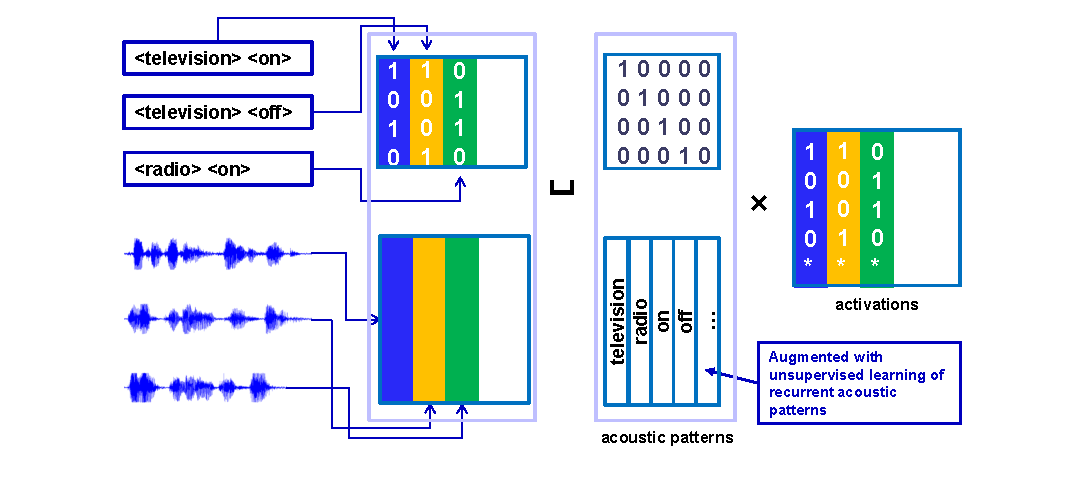
\includegraphics[width=1.3\linewidth]{NMF_fig.eps}
		
		\large{
			\begin{align}
				(\bs{W}, \bs{H}) = \underset{(\bs{W}, \bs{H})}{\operatorname{arg\ max\ }} \log P(\bs{V} \vert \bs{W}, \bs{H}) \nonumber
			\end{align}
		}
		\large{
			Problems to be solved:
			\begin{itemize}
				\item Full batch learning: all data available during training
				\item Fixed dictionary size: chosen a priori and remains constant
			\end{itemize}	
		}	
	}
}\hbs
\rframe{.32}{1}
{
	\rtextbox{.32}{.58}{4. Incremental ARD}
	{%
		\Large{ARD: Automatic Relevance Determination}
		\vspace{1cm}
		
		\center{
		\begin{tikzpicture}
			\node[element] (grow) at (0,0) {\textbf{Naively grow dictionary}};
			\node[element] (update) at (7,-3) {\textbf{Update Model}};
			\node[element] (remove) at (14,-6) {\textbf{Remove irrelevant words}};
			\draw[->, line width=3pt] (grow) -- (update);
			\draw[->, line width=3pt] (update) -- (remove);
			\draw[->, line width=3pt] (remove) -- (0,-6) --  (grow);
		\end{tikzpicture}}
		
		\vspace{1cm}
		
		
		\begin{minipage}{\linewidth}
			\Large
			\begin{align}
				(\bs{W}, \bs{H}, \bs{\nu}) = \underset{(\bs{W}, \bs{H}, \bs{\nu})}{\operatorname{arg\ max\ }} \log P(\bs{W}, \bs{H}, \bs{\nu}\vert\bs{V}) \nonumber
			\end{align}
			
			\vspace{1cm}
			
			$\bs{\nu}$: Relevance of each word in the dictionary (one parameter per dictionary element)
			
			\begin{align}
				P(\bs{W}, \bs{H}, \bs{\nu}\vert\bs{V}) = \frac{\textcolor{red}{P(\bs{V} \vert \bs{W}, \bs{H})}\textcolor{green}{P(\bs{W})}\textcolor{blue}{P(\bs{H} \vert \bs{\nu})}\textcolor{purple}{P(\bs{\nu})}}{P(\bs{V})} \nonumber
			\end{align}
		\end{minipage}
		
		\Large{
			\begin{itemize}
				\item \textcolor{red}{Data likelihood: Model data well}
				\item \textcolor{green}{Dictionary prior: Remember the dictionary}
				\item \textcolor{blue}{Activation prior: Only activate relevant words}
				\item \textcolor{purple}{Relevance prior: Remember word relevance}
			\end{itemize}	
		}
	
	}\vbs
	\rtextbox{.32}{.27}{5. Experiments}
	{
		\vspace{-2cm}
		\Large{
			\begin{itemize}
				\item \texttt{Syncom}: Commands for various electronic devices
				\item 5 users, 3 sets, 16 commands, 5 repetitions
				\item Sets: same action, different command
				\item Update model with batches of 16 randomly chosen examples
				\item Test on remaining unseen data
				\item Simulate a sudden change in behaviour
				\item With ARD (ARD) vs without ARD (base)
			\end{itemize}
		}
	}\vbs
	\rtextbox{.32}{.15}{7. Conclusions}
	{
		\vspace{-2cm}
		\Large{\begin{itemize}
			\item Dictionary grows and shrinks
			\item Flexibility changing behaviour
			\item Add new + remove old $\leftrightarrow$ adapt old to new
		\end{itemize}}
	}
}\hbs
\rframe{.38}{1}
{
	\rtextbox{.38}{1}{6. Results}
	{
\begin{minipage}{\linewidth}
\centering
\large
\textbf{Label accuracy} for several test scenarios in function of number of presented batches\\
\Large
\vspace{1cm}
\begin{tabular}{|c|cc|cc|cc|cc|}
\hline
 & \multicolumn{2}{c|}{3-0} & \multicolumn{2}{c|}{2-1} & \multicolumn{2}{c|}{1-2} & \multicolumn{2}{c|}{1-1}\\
 & ARD & base & ARD & base & ARD & base & ARD & base\\
 \hline
$1$ & $55.0$ & $54.0$ & $57.9$ & $56.6$ & $69.1$ & $68.6$ & $68.6$ & $68.8$\\
$2$ & $71.9$ & $69.0$ & $76.3$ & $72.9$ & $88.7$ & $87.5$ & $89.1$ & $84.7$\\
$3$ & $79.7$ & $76.3$ & $85.2$ & $80.4$ & $95.3$ & $92.1$ & $95.8$ & $91.2$\\
$4$ & $84.4$ & $80.6$ & $89.1$ & $84.3$ & $98.0$ & $93.1$ & $97.8$ & $93.1$\\
\cline{6-9}
$5$ & $87.8$ & $83.1$ & $92.0$ & $86.6$ & $64.2$ & $62.2$ & $64.0$ & $61.5$\\
$6$ & $90.2$ & $84.6$ & $93.0$ & $88.3$ & $76.2$ & $70.8$ & $80.8$ & $74.7$\\
$7$ & $90.4$ & $85.6$ & $93.8$ & $89.2$ & $83.1$ & $76.7$ & $90.1$ & $82.2$\\
$8$ & $91.3$ & $86.4$ & $94.6$ & $90.3$ & $86.7$ & $80.3$ & $93.8$ & $86.4$\\
$9$ & $92.6$ & $87.1$ & $94.4$ & $91.3$ & $90.1$ & $83.4$ & $95.6$ & $88.1$\\
\cline{4-5}
$10$ & $92.1$ & $88.3$ & $73.5$ & $70.8$ & $92.6$ & $85.0$ &  & \\
$11$ & $91.0$ & $87.7$ & $84.1$ & $77.4$ & $93.4$ & $86.2$ &  & \\
$12$ & $92.1$ & $87.6$ & $89.8$ & $82.4$ & $94.2$ & $87.3$ &  & \\
$13$ & $91.5$ & $88.0$ & $93.5$ & $85.3$ & $94.0$ & $88.3$ &  & \\
$14$ & $91.5$ & $86.7$ & $95.7$ & $86.7$ & $94.4$ & $88.9$ &  & \\
\hline
\end{tabular}
\end{minipage}
\vspace{2cm}

\begin{minipage}{\linewidth}
\centering
\large
\textbf{Dictionary size} for several test scenarios in function of number of presented batches\\
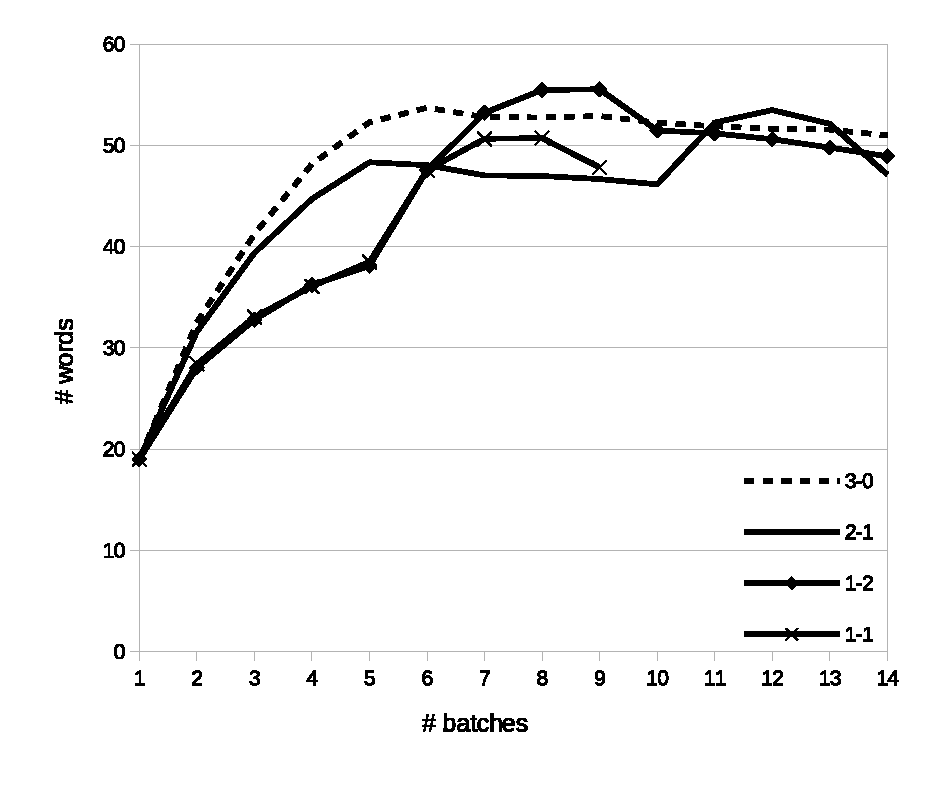
\includegraphics[width=0.8\linewidth]{OrdEng.eps}
\end{minipage}

\large{
\begin{itemize}
\item Before Change: performance increases, dictionary grows and stabilises
\item At Change: performance drop
\item Immediately after change: new words added to dictionary
\item After change:  performance recovery, old words removed
\end{itemize}
}


	}\vbs
	
}



\end{document}
